\documentclass[12pt,letterpaper]{article}

\usepackage{fancyhdr,fancybox}
\usepackage{wrapfig}

%% Useful packages
\usepackage{amssymb, amsmath, amsthm} 
%\usepackage{graphicx}  %%this is currently enabled in the default document, so it is commented out here. 
\usepackage{calrsfs}
\usepackage{braket}
\usepackage{mathtools}
\usepackage{lipsum}
\usepackage{tikz}
\usetikzlibrary{cd}
\usepackage{verbatim}
%\usepackage{ntheorem}% for theorem-like environments
\usepackage{mdframed}%can make highlighted boxes of text
%Use case: https://tex.stackexchange.com/questions/46828/how-to-highlight-important-parts-with-a-gray-background
\usepackage{wrapfig}
\usepackage{centernot}
\usepackage{subcaption}%\begin{subfigure}{0.5\textwidth}
\usepackage{pgfplots}
\pgfplotsset{compat=1.13}
\usepackage[colorinlistoftodos]{todonotes}
\usepackage[colorlinks=true, allcolors=blue]{hyperref}
\usepackage{xfrac}					%to make slanted fractions \sfrac{numerator}{denominator}
\usepackage{enumitem}            
    %syntax: \begin{enumerate}[label=(\alph*)]
    %possible arguments: f \alph*, \Alph*, \arabic*, \roman* and \Roman*
\usetikzlibrary{arrows,shapes.geometric,fit}

\DeclareMathAlphabet{\pazocal}{OMS}{zplm}{m}{n}
%% Use \pazocal{letter} to typeset a letter in the other kind 
%%  of math calligraphic font. 

%% This puts the QED block at the end of each proof, the way I like it. 
\renewenvironment{proof}{{\bfseries Proof}}{\qed}
\makeatletter
\renewenvironment{proof}[1][\bfseries \proofname]{\par
  \pushQED{\qed}%
  \normalfont \topsep6\p@\@plus6\p@\relax
  \trivlist
  %\itemindent\normalparindent
  \item[\hskip\labelsep
        \scshape
    #1\@addpunct{}]\ignorespaces
}{%
  \popQED\endtrivlist\@endpefalse
}
\makeatother

%% This adds a \rewnewtheorem command, which enables me to override the settings for theorems contained in this document.
\makeatletter
\def\renewtheorem#1{%
  \expandafter\let\csname#1\endcsname\relax
  \expandafter\let\csname c@#1\endcsname\relax
  \gdef\renewtheorem@envname{#1}
  \renewtheorem@secpar
}
\def\renewtheorem@secpar{\@ifnextchar[{\renewtheorem@numberedlike}{\renewtheorem@nonumberedlike}}
\def\renewtheorem@numberedlike[#1]#2{\newtheorem{\renewtheorem@envname}[#1]{#2}}
\def\renewtheorem@nonumberedlike#1{  
\def\renewtheorem@caption{#1}
\edef\renewtheorem@nowithin{\noexpand\newtheorem{\renewtheorem@envname}{\renewtheorem@caption}}
\renewtheorem@thirdpar
}
\def\renewtheorem@thirdpar{\@ifnextchar[{\renewtheorem@within}{\renewtheorem@nowithin}}
\def\renewtheorem@within[#1]{\renewtheorem@nowithin[#1]}
\makeatother

%% This makes theorems and definitions with names show up in bold, the way I like it. 
\makeatletter
\def\th@plain{%
  \thm@notefont{}% same as heading font
  \itshape % body font
}
\def\th@definition{%
  \thm@notefont{}% same as heading font
  \normalfont % body font
}
\makeatother

%===============================================
%==============Shortcut Commands================
%===============================================
\newcommand{\ds}{\displaystyle}
\newcommand{\B}{\mathcal{B}}
\newcommand{\C}{\mathbb{C}}
\newcommand{\F}{\mathbb{F}}
\newcommand{\N}{\mathbb{N}}
\newcommand{\R}{\mathbb{R}}
\newcommand{\Q}{\mathbb{Q}}
\newcommand{\T}{\mathcal{T}}
\newcommand{\Z}{\mathbb{Z}}
\renewcommand\qedsymbol{$\blacksquare$}
\newcommand{\qedwhite}{\hfill\ensuremath{\square}}
\newcommand*\conj[1]{\overline{#1}}
\newcommand*\closure[1]{\overline{#1}}
\newcommand*\mean[1]{\overline{#1}}
%\newcommand{\inner}[1]{\left< #1 \right>}
\newcommand{\inner}[2]{\left< #1, #2 \right>}
\newcommand{\powerset}[1]{\pazocal{P}(#1)}
%% Use \pazocal{letter} to typeset a letter in the other kind 
%%  of math calligraphic font. 
\newcommand{\cardinality}[1]{\left| #1 \right|}
\newcommand{\domain}[1]{\mathcal{D}(#1)}
\newcommand{\image}{\text{Im}}
\newcommand{\inv}[1]{#1^{-1}}
\newcommand{\preimage}[2]{#1^{-1}\left(#2\right)}
\newcommand{\script}[1]{\mathcal{#1}}


\newenvironment{highlight}{\begin{mdframed}[backgroundcolor=gray!20]}{\end{mdframed}}

\DeclarePairedDelimiter\ceil{\lceil}{\rceil}
\DeclarePairedDelimiter\floor{\lfloor}{\rfloor}

%===============================================
%===============My Tikz Commands================
%===============================================
\newcommand{\drawsquiggle}[1]{\draw[shift={(#1,0)}] (.005,.05) -- (-.005,.02) -- (.005,-.02) -- (-.005,-.05);}
\newcommand{\drawpoint}[2]{\draw[*-*] (#1,0.01) node[below, shift={(0,-.2)}] {#2};}
\newcommand{\drawopoint}[2]{\draw[o-o] (#1,0.01) node[below, shift={(0,-.2)}] {#2};}
\newcommand{\drawlpoint}[2]{\draw (#1,0.02) -- (#1,-0.02) node[below] {#2};}
\newcommand{\drawlbrack}[2]{\draw (#1+.01,0.02) --(#1,0.02) -- (#1,-0.02) -- (#1+.01,-0.02) node[below, shift={(-.01,0)}] {#2};}
\newcommand{\drawrbrack}[2]{\draw (#1-.01,0.02) --(#1,0.02) -- (#1,-0.02) -- (#1-.01,-0.02) node[below, shift={(+.01,0)}] {#2};}

%***********************************************
%**************Start of Document****************
%***********************************************
 %find me at /home/trevor/texmf/tex/latex/tskpreamble_nothms.tex
%===============================================
%===============Theorem Styles==================
%===============================================

%================Default Style==================
\theoremstyle{plain}% is the default. it sets the text in italic and adds extra space above and below the \newtheorems listed below it in the input. it is recommended for theorems, corollaries, lemmas, propositions, conjectures, criteria, and (possibly; depends on the subject area) algorithms.
\newtheorem{theorem}{Theorem}
\numberwithin{theorem}{section} %This sets the numbering system for theorems to number them down to the {argument} level. I have it set to number down to the {section} level right now.
\newtheorem*{theorem*}{Theorem} %Theorem with no numbering
\newtheorem{corollary}[theorem]{Corollary}
\newtheorem*{corollary*}{Corollary}
\newtheorem{conjecture}[theorem]{Conjecture}
\newtheorem{lemma}[theorem]{Lemma}
\newtheorem*{lemma*}{Lemma}
\newtheorem{proposition}[theorem]{Proposition}
\newtheorem*{proposition*}{Proposition}
\newtheorem{problemstatement}[theorem]{Problem Statement}


%==============Definition Style=================
\theoremstyle{definition}% adds extra space above and below, but sets the text in roman. it is recommended for definitions, conditions, problems, and examples; i've alse seen it used for exercises.
\newtheorem{definition}[theorem]{Definition}
\newtheorem*{definition*}{Definition}
\newtheorem{condition}[theorem]{Condition}
\newtheorem{problem}[theorem]{Problem}
\newtheorem{example}[theorem]{Example}
\newtheorem*{example*}{Example}
\newtheorem*{counterexample*}{Counterexample}
\newtheorem*{romantheorem*}{Theorem} %Theorem with no numbering
\newtheorem{exercise}{Exercise}
\numberwithin{exercise}{section}
\newtheorem{algorithm}[theorem]{Algorithm}

%================Remark Style===================
\theoremstyle{remark}% is set in roman, with no additional space above or below. it is recommended for remarks, notes, notation, claims, summaries, acknowledgments, cases, and conclusions.
\newtheorem{remark}[theorem]{Remark}
\newtheorem*{remark*}{Remark}
\newtheorem{notation}[theorem]{Notation}
\newtheorem*{notation*}{Notation}
%\newtheorem{claim}[theorem]{Claim}  %%use this if you ever want claims to be numbered
\newtheorem*{claim}{Claim}


%%
%% Page set-up:
%%
\pagestyle{empty}
\lhead{\textsc{221 - Topology} \\ } %=================UPDATE THIS=================%
\rhead{\textsc{McCammond, Winter 2019} \\ Trevor Klar}
%\chead{\Large\textbf{A New Integration Technique \\ }}
\renewcommand{\headrulewidth}{0pt}
%
\renewcommand{\footrulewidth}{0pt}
%\lfoot{
%Office: \quad \quad \, M 2-3 \, \, SH 6431x \\
%Math Lab: \, W 12-2 \, SH 1607
%}
%\rfoot{trevorklar@math.ucsb.edu}


\setlength{\parindent}{0in}
\setlength{\textwidth}{7in}
\setlength{\evensidemargin}{-0.25in}
\setlength{\oddsidemargin}{-0.25in}
\setlength{\parskip}{.5\baselineskip}
\setlength{\topmargin}{-0.5in}
\setlength{\textheight}{9in}

\setlist[enumerate,1]{label=\textbf{\arabic*.}}

\begin{document}
\pagestyle{fancy}
\begin{center}
{\Large Homework 3}%=================UPDATE THIS=================%
\end{center}

\begin{enumerate}
\setcounter{enumi}{14}
\item Enumerate all the subcomplexes of $S^\infty$, with the cell structure on $S^\infty$ that has $S^n$ as its $n$ skeleton.

\answer The cell structure $S^\infty$ that has $S^n$ as its $n$ skeleton is given by building each $k$-th sphere on top of the $k-$th sphere: so beginning with $S^0$ (two points), we attach two $e^1$s by attaching their boundaries to what has already been built. 
\jpg{width=0.8\textwidth}{hw3-p15-1}

Thus a diagram of the attaching maps can be drawn as follows:
\jpg{width=0.8\textwidth}{hw3-p15-2}

Now we will show that any subcomplex is either a hemisphere or a sphere, and the following list enumerates them:
$$\left\lbrace 
\langle{e^0_a}\rangle,\; \langle{e^0_b}\rangle,\; \left(\langle{e^0_a}\rangle \cup \langle{e^0_b}\rangle\right),\;
\langle{e^1_a}\rangle,\; \langle{e^1_b}\rangle,\; \left(\langle{e^1_a}\rangle \cup \langle{e^1_b}\rangle\right),\; \dots
\right\rbrace$$
where $\langle e^i_\delta \rangle$ denotes the subcomplex generated by $e^i_\delta$. Observe that for any single cell $e^n_\delta\in S^\infty$, $\langle e^n_\delta \rangle$ is a hemisphere, since each $e^i$ is attached to both $e^{i-1}$ cells. 
Thus to examine the subcomplex generated by any finite collection of cells $E$, we need only consider the cells of highest dimension, namely $e^n_a$ and/or $e^n_b$. 
If only one of $e^n_a, e^n_b\in E$, then we have an $n$-hemisphere. Otherwise, we have the $n$-sphere. 
Now if $E$ a collection of cells of $S^\infty$ is infinite, then $\langle E\rangle = S^\infty$ since for any $e^n_\delta\in S^\infty$, there is some $e^k_\gamma\in E$ with $k>n$. \qed

\pagebreak
\item Show that $S^\infty$ is contractible. 
\begin{proof}
We can actually construct a deformation retraction of $S^\infty$ to $e^0_a$ as a countable concatenation of homotopies. 
	\begin{enumerate}[label=(\arabic*)]
	\item Let $F_1$ be the homotopy which deformation retracts $\langle e^1_a \rangle$ (the $a$-th semicircle) to $e^0_a$. This has the effect of retracting all of $S^0$ to $e^0_a$. 
\jpg{width=0.33\textwidth}{hw3-p16-1}
Note that any point in $S^\infty$ except $e^0_a$ can move to accomplish this, but we constrain points  $S^n$ to never leave $S^n$ for all $n>0$. Here we draw more dimensions to illustrate:
\jpg{width=0.33\textwidth}{hw3-p16-2}

	\item[$(i)$] For each $i\geq2$, let $F_i$ be the homotopy which deformation retracts $\langle e^i_a \rangle$ (the $a$-th i-hemisphere) to $e^0_a$. We know we can do this because each hemisphere is a disk which contains $e^0_a$. This has the effect of retracting all of $S^{i-1}$ to $e^0_a$. 
	\end{enumerate}
Now we concatenate all of these homotopies, allotting time $\frac{1}{2^i}$ for each $F_i$, so that they are all completed as $t$ goes from 0 to 1. Every $S^i\subset S^\infty$ is deformation retracted to the point $e^0_a$ by the time $t=1-2^{-(i+1)}$, so $S^\infty$ is contractible. 
\end{proof}

\pagebreak
\setcounter{enumi}{17}
\item Show that $S^1 * S^1 = S^3$, and more generally $S^m * S^n = S^{m+n+1}$. 
\begin{proof}
By definition, $S^m*S^n$ is a shape which has an $m$-sphere on one end, an $n$-sphere on the other end, and everywhere in between is shaped like a $S^m\times S^n$. Following is an illustration when $m=n=1$:
\jpg{width=0.8\textwidth}{hw3-p18-1}
We can consider two halves of this shape, glued together on their boundaries. Since every point in the $m$-sphere is connected to every point in the $n$-sphere, we can see this as 
$$ S^m\times C(S^n)\bigsqcup_{S^m\times S^n} C(S^m)\times S^n$$
which is the same as 
$$ S^m\times D^{n+1}\bigsqcup_{S^m\times S^n} D^{m+1}\times S^n$$
(there's a really cool picture of interlocking solid tori which doesn't turn out to be helpful for what we want to prove here, so I've left it out). 

Now observe that the unit sphere $S^{m+n+1}\in\R^{m+n+2}$ is the locus of points such that
$$\overbrace{x_1^2+\dots+x_{m+1}^2}^{m+1} + \overbrace{x_{m+2}^2+\dots+x_{m+n+2}^2}^{n+1}=1$$
or equivalently, 
\begin{equation*}
x_1^2+\dots+x_{m+1}^2 = t \quad \text{ and } \quad x_{m+2}^2+\dots+x_{m+n+2}^2=(1-t) \quad \text{ for } \quad t\in[0,1].
\end{equation*}
which is the same as 
\begin{equation}
x_1^2+\dots+x_{m+1}^2 = t \quad \text{ and } \quad x_{m+2}^2+\dots+x_{m+n+2}^2=(1-t) \quad \text{ for } \quad t\in[0,\tfrac{1}{2}].
\end{equation}
\begin{center}
together with 
\end{center}
\begin{equation}
x_1^2+\dots+x_{m+1}^2 = (1-s) \quad \text{ and } \quad x_{m+2}^2+\dots+x_{m+n+2}^2=s \quad \text{ for } \quad s\in[0,\tfrac{1}{2}].
\end{equation}
where we attach (1) and (2) along the set where $s=t=\frac{1}{2}$ (note how the equations agree in that case). 

What regions do these equations describe? First consider (1). In the left hand equation, $t$ determines the radius of an $m-$sphere, so letting $t$ vary gives an $m+1$ disk. Using $t$ in the right-hand equation gives an $n$-sphere whose radius is a function of $t$. Thus, for every point in an $m+1$ disk of radius $\sqrt{\tfrac{1}{2}}$, we can choose any point in an $n$-sphere to satisfy (1). Thus (1) determines a region which is the shape of $D^{m+1}\times S^n$.

Using similar reasoning, we can see that (2) determines a region which is the shape of ${S^m\times D^{n+1}}$. Finally, we observe that for $t=s=\frac{1}{2}$, both equations determine the same set of points $S^m\times S^n$. Thus an $m+n+1$-sphere is the same homotopy type as $$ {S^m\times D^{n+1}\bigsqcup_{S^m\times S^n} D^{m+1}\times S^n},$$ which is $S^m*S^n$. \end{proof}

\item Show that the space obtained from $S^2$ by attaching $n$ 2--cells along any collection of $n$ circles in $S^2$  is homotopy equivalent to the wedge sum of $n + 1$ 2--spheres.
\begin{proof}
Any circle in $S^2$ divides $S^2$ into two 2-disks which are contractible. For every one of these circles, call part of $S^2$ the inside of this circle and contract it to a point. Then move the attaching maps so all the spheres are attached to each other at the same point, and we're done. 
\jpg{width=0.8\textwidth}{hw3-p19-1}
\end{proof}
\end{enumerate}

\pagebreak
\vspace*{-3ex}
\begin{minipage}{0.8\linewidth}
\begin{enumerate}[resume]
\item Show that the subspace $X \subset \R^3$ formed by a Klein bottle intersecting itself in a circle, as shown in the figure, is homotopy equivalent to $S^1\vee S^1  \vee S^2$. \\\\
\end{enumerate}
\end{minipage}
\begin{minipage}{0.2\linewidth}
\raisebox{-\height}{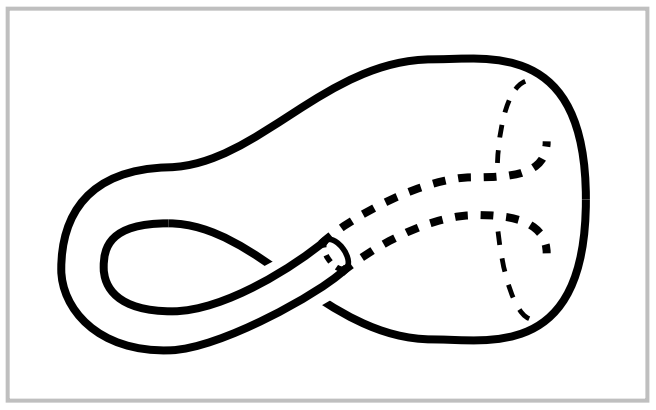
\includegraphics[width=\linewidth]{hw3-p20-1}}
\end{minipage}

\begin{enumerate}
\setcounter{enumi}{19}
\item[\phantom{19.}]
\vspace*{-5ex}
\begin{proof}
See the following figure. 
\jpg{width=0.8\textwidth}{hw3-p20-2}
\vspace*{-2ex}Observe that contracting the blue disk in (1) to a point gives us (2), and contracting both blue 1-cells in (3) to a point also gives (2), so those three figures are homotopy equivalent. The green lines show how the attaching maps for the top and bottom points are homotopic to attaching maps which attach the blue 1-cells' endpoints all to the same point, so ${(3) \simeq (4)}$. 
\end{proof}
\end{enumerate}

\vfill

Collaborators:
\begin{enumerate}
\setcounter{enumi}{14}
\item 

\item 

\setcounter{enumi}{17}
\item Kyle Hansen, Zach Wagner, Paige Hillen

\item Zach Wagner

\item Kyle Hansen, Zach Wagner
\end{enumerate}
\end{document}



